\documentclass{beamer}

\usepackage{listings}  % Package to include python syntax code
\usepackage{color} % Package to include colors for syntax highlighting
\usepackage{graphicx}  % Package to include images
\usepackage{hyperref}  % Hyperlinks
\usepackage{tikz}

\lstset{  % Settings for listings package
backgroundcolor=\color{cyan!10},  % Includes a light blue background color
numbers=left,  % Includes line numbers
keywordstyle=\bfseries\color{green!40!black},  % Bold and color green for keywords
identifierstyle=\color{blue},  % Other words are colored blue
stringstyle=\color{orange},  % Strings are orange
showstringspaces=false  % Don't show spaces in strings
}

\setbeamertemplate{navigation symbols}{}  % Remove navigation symbols

\title{Computing for Mathematics: Week 1}
\date{}


\begin{document}

\frame{
\titlepage
}

\frame{
\frametitle{Vince Knight}

\begin{itemize}
    \item Office: M1.25
    \item email: knightva@cf.ac.uk
    \item Office hours: Thursday 1300 - 1500
\end{itemize}

}

\frame{
\href{https://www.youtube.com/watch?v=qEr6mcgdsmI}{
$$\begin{pmatrix}
(0,0) & (-1,1) & (1,-1)\\
(1,-1) & (0,0) & (-1,1)\\
(1,-1) & (-1,1) & (0,0)\\
\end{pmatrix}$$}
}

\frame{
\frametitle{Programming and Mathematics}

There are various areas in which computers are of major importance to Mathematicians:

\begin{itemize}
\item Computer assisted proofs;
\item Implementation of mathematics;
\item Computer generated proofs;
\item Everyday mathematics.
\end{itemize}

}

\frame{
\frametitle{Computer assisted proofs}

\begin{center}

\begin{tikzpicture}

\only<1>{
\node (A) [circle, draw] at (-.5,2) {0};
\node (B) [circle, draw] at (0,1) {1};
\node (C) [circle, draw] at (1.5,2) {2};
\node (D) [circle, draw] at (-.5,0) {3};
\node (E) [circle, draw] at (2,.7) {4};
}

\only<2>{
\node (A) [circle, draw, fill=blue] at (-.5,2) {0};
\node (B) [circle, draw] at (0,1) {1};
\node (C) [circle, draw] at (1.5,2) {2};
\node (D) [circle, draw] at (-.5,0) {3};
\node (E) [circle, draw] at (2,.7) {4};
}

\only<3>{
\node (A) [circle, draw, fill=blue] at (-.5,2) {0};
\node (B) [circle, draw, fill=green] at (0,1) {1};
\node (C) [circle, draw] at (1.5,2) {2};
\node (D) [circle, draw] at (-.5,0) {3};
\node (E) [circle, draw] at (2,.7) {4};
}

\only<4>{
\node (A) [circle, draw, fill=blue] at (-.5,2) {0};
\node (B) [circle, draw, fill=green] at (0,1) {1};
\node (C) [circle, draw, fill=red] at (1.5,2) {2};
\node (D) [circle, draw, fill=red] at (-.5,0) {3};
\node (E) [circle, draw] at (2,.7) {4};
}

\only<5-6>{
\node (A) [circle, draw, fill=blue] at (-.5,2) {0};
\node (B) [circle, draw, fill=green] at (0,1) {1};
\node (C) [circle, draw, fill=red] at (1.5,2) {2};
\node (D) [circle, draw, fill=red] at (-.5,0) {3};
\node (E) [circle, draw, fill=gray] at (2,.7) {4};
}
\draw (A) -- (C);
\draw (A) -- (B);
\draw (A) -- (D);
\draw (A) -- (E);
\draw (B) -- (C);
\draw (B) -- (E);
\draw (B) -- (D);
\draw (E) -- (D);
\draw (E) -- (C);
\end{tikzpicture}
\end{center}

\begin{itemize}
\onslide<5-6>{
\item `4 colour theorem': \textbf{Any map can be coloured using 4 colours.\\}
}

\onslide<6>{

\item Proved in 1976 by Kenneth Appel and Wolfgang Haken:
\begin{center}
\framebox{Used computers to check 1936 particular cases.}
\end{center}

}
\end{itemize}
}

\frame{\frametitle{Risk boards}
\begin{center}
    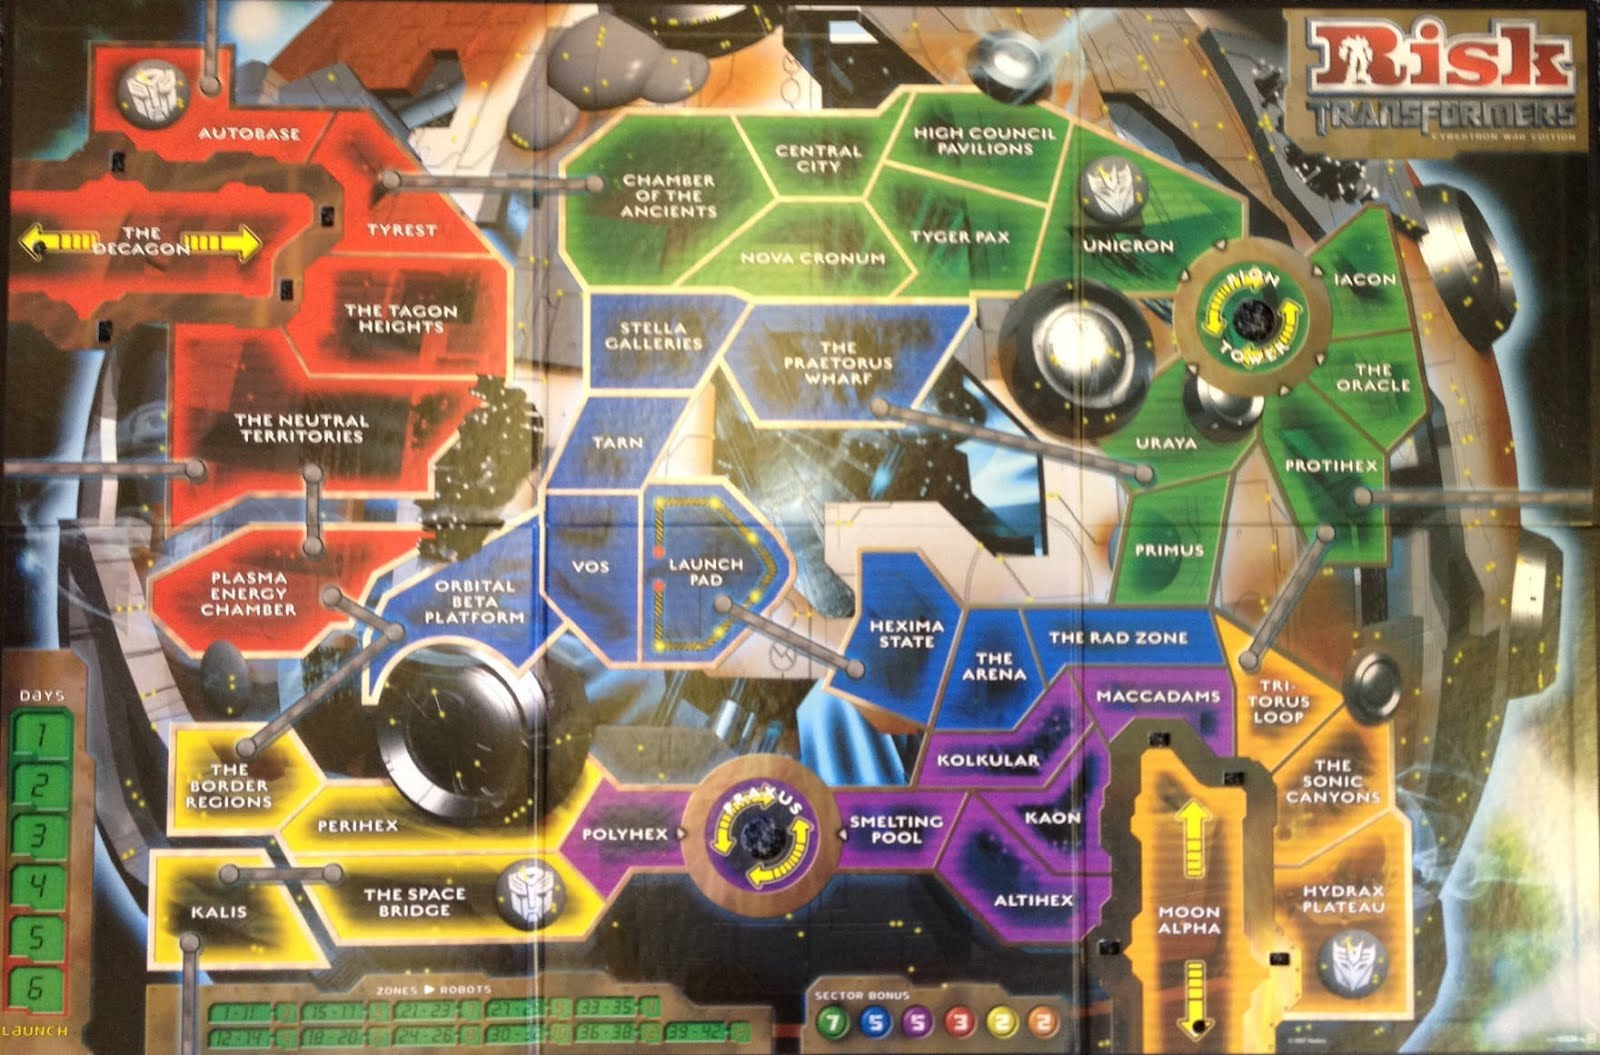
\includegraphics[width=10cm]{./images/W01-img03.png}
\end{center}
}

\frame{
\frametitle{Computer assisted proofs}
How to pack 3 dimensional spheres?

\begin{itemize}
\item In 1611 Kepler conjectured the best possible way.
\item Proof in 1998 by Hales which involved a computer to minimize a function of 150 variables (100,000 times).
\item \textbf{Also} involved a 100 page paper for the 'non computer assisted aspects'.
\pause
\item Referees are 99\% sure.
\end{itemize}
}

\frame{
\frametitle{Implementation of mathematics}
Here at Cardiff Dr Leanne Smith studied the best way to locate ambulances in Wales. This took in to account:

\begin{itemize}
\item Queues;
\item Survival probabilities of patients;
\item Time of the day...
\end{itemize}

\href{http://www.youtube.com/watch?v=mMFCmd0fwjY&feature=youtu.be}{Once the mathematics was done a computer program was built to be able to demonstrate to the Welsh Ambulance Trust.}
}

\frame{
\frametitle{Computer generated proofs}
\begin{center}
\href{http://goo.gl/tsdOiQ}{Timothy Gowers}
\end{center}
\pause
Theorem: Let $X$ and $Y$ be sets, let $f: X \to Y$ be an injection and let $A$ and $B$ be subsetsof $X$. Then $f(A)\cap f(B)\subset f(A\cap B)$.\\

\vspace{1cm}
\pause
Proof: Take $x\in f(A)\cap f(B)$. So there is some $y\in A$ and $z\in B$ such that $f(y)=f(z)=x$. As $f$ is injective, $y$ and $z$ are equal. So $y\in A\cap B$. So $x=f(y)\in f(A\cap B)$.

\pause
\vspace{1cm}
The above is an example of a computer generated proof. \textbf{You do not need to know any of this!}

}

\begin{frame}[fragile]
\frametitle{Everyday mathematics}
Everyday mathematicians might need to calculate an integral for a bigger project. This is some Sage code to calculate an integral:

\begin{lstlisting}[language=python]
integrate(x ^ 3, x)
\end{lstlisting}

which returns:

$$\frac{x^4}{4}$$
\end{frame}

\frame{
\frametitle{What we will learn}
\begin{itemize}
\item Python: general purpose programming language (Weeks 1-5).
\item Sage: mathematics package (based on Python) (Weeks 5-9).
\item \LaTeX:\; a package for writing mathematics (Week 10).
\end{itemize}
}

\frame{
\frametitle{Flipped classrooms}
\pause
\begin{center}
    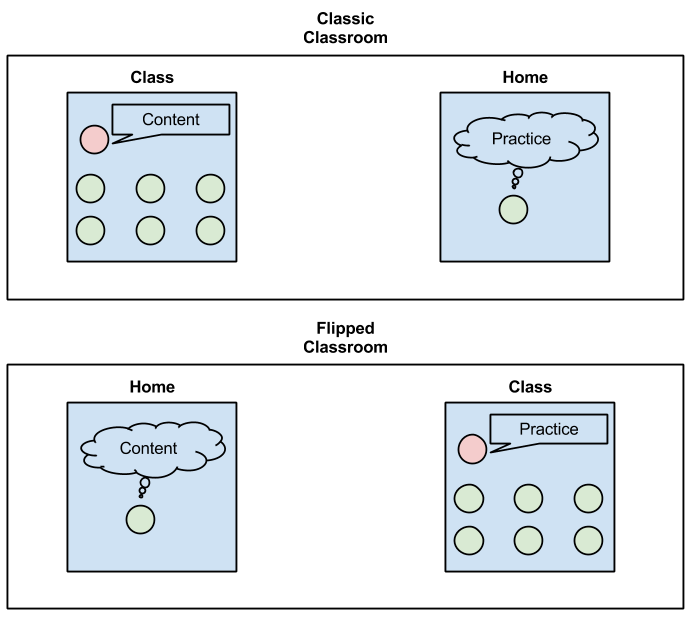
\includegraphics[width=8cm]{./images/W01-img01.png}
\end{center}
}

\frame{
\frametitle{Labs and `Tickables'}
\begin{itemize}
\item Every week you have 2 computer lab sessions.
\item You have until the end of the second lab session to complete all exercises marked as `TICKABLE'.
\item You will need to work on these outside of the lab sessions.
\end{itemize}
}

\frame{
\frametitle{Resources}
\begin{center}
%\href{http://drvinceknight.github.io/Computing_for_mathematics/}{drvinceknight.github.io/Computing_for_mathematics/}
\href{http://www.vincent-knight.com/home/teaching/computing-for-mathematics}{http://www.vincent-knight.com/home/teaching/computing-for-mathematics}
\end{center}
}

\end{document}
